\documentclass{article}
\usepackage[utf8]{inputenc}
\usepackage{graphicx}

\begin{document}
\title{Prerequisite test of the Computer Vision course at the
  University of Helsinki in May 2018}

\author{\emph{your name here}}
\maketitle

\newpage

\section{Introduction}

The purpose of this document and the prerequisite test for the
computer vision course is, first, to verify that all participants have
a functioning software setup in their computers when the course
starts.  Second, it makes sure that the participants are able to
compose the results of their home works into PDF reports and to submit
them to the lecturer.

In general, the results of this prerequisite test and the daily home
work reports can be written by using also any other software than
pdf\LaTeX{}.  The only thing that matters is that the submitted report
is in a single PDF file and contains the used program codes and
generated images in a readable and clear form.

The aim is, that you compile and run the two included programs
\texttt{test.cc} (written in C++) and \texttt{test.py} (written in
Python).  Running them successfully will produce four images that will
be included in the prerequisite report that you email to the lecturer.
 
If you encounter technical problems in completing the prerequisite
test, you can contact the course teaching assistant Gür Ersalan by
phone 041 807 0887 or by email \texttt{muzaffer.ersalan@helsinki.fi}
and ask support from him.

\textbf{Deadline for the submission is Friday 11.5.2018 at 23:59 o'clock!}

\section{Instructions}
\label{sec:running}

\subsection{Copy the report template}

The distributed ZIP file contains this file in both PDF and
pdf\LaTeX{} source formats.  The source code of the document is stored
in \texttt{your\_name\_report\_0.tex}.  Copy it to a new file whose
name contains your own name.  (The daily home work reports you can
create from this same example by replacing the ``0'' with numbers
``1''\ldots``4''.)

Read what follows in this document and modify it by answering to the
stated questions and by doing the other requested updates!


\subsection{Fill in the statistics}

First some statistics.  Answer to the following questions by replacing
the lecturer's answers with your own:

\begin{itemize}
\item What is your operating system? \emph{Linux}
\item What is its distribution and/or release? \emph{Ubuntu 17.10}
\item Have you used Python before? \emph{Yes}
\item Have you used C++ before? \emph{Yes}
\item Have you used OpenCV before? \emph{Yes}
\item Have you taken a course in image processing or computer vision? \emph{Yes}
\end{itemize}


\subsection{Run \texttt{test.cc}}

You should be able to run \texttt{test.cc} by first compiling and
linking it with the GNU C++ compiler \texttt{g++} and then executing
the resulting \emph{a.out} executable.

This is an example of command lines to perform the compilation and to
run the created executable:

{\small
\begin{verbatim}
g++ test.cc -lopencv_core -lopencv_imgproc -lopencv_highgui -lopencv_imgcodecs -lopencv_plot
./a.out
\end{verbatim}
}

At least the following software packages need to be installed for the
compilation and linking to succeed:

\begin{itemize}
\item g++
\item libopencv-core-dev
\item libopencv-highgui-dev
\item libopencv-imgproc-dev
\item libopencv-imgcodecs-dev
\item \emph{(add the extra packages you had to install here\ldots)}
\end{itemize}

Complete the above list with the possible extra packages you needed
to install to get the code run.

Note: The OpenCV class \texttt{cv::plot::Plot2d} has changed slightly
between OpenCV releases 3.1.0 and 3.4.1.  The code in \texttt{test.cc}
expects the version is 3.1.0, but the newer interface can be taken
into use by changing the out-commented lines.

Running the code will first show a color image of a football player.
Pressing a key while input focus is in the image or destroying the
window will show a related greyscale image.  Finally you should see a
yellow plot on black background.  Closing that plot will end the run.

During the run you should have seen the following output:

\begin{verbatim}
x.y.z
rows=342 cols=548 channels=3 type=16 (type 16 means CV_8UC3)
rows=342 cols=548 channels=1 type=0 (type 0 means CV_8UC1)
\end{verbatim}

Also, two new image files \texttt{green.jpg} and
\texttt{projection.png} should have appeared.

Answer to the following questions:

\begin{itemize}
\item What was \texttt{x.y.z} (OpenCV version) in your output? \emph{your answer here} 
\item Did you see the two images and one plot? \emph{your answer here} 
\end{itemize}


\subsection{Run \texttt{test.py}}

You should be able to run \texttt{test.py} by executing it from
Linux's command line or by some other similar means.  At least the
following software packages need to be installed for it to work:

\begin{itemize}
\item python3
\item python3-opencv
\item \emph{(add the extra packages you had to install here\ldots)}
\end{itemize}

Complete the above list with the possible extra packages you needed
to install to get the code run.

Running the code will first show a color image of a football player.
Pressing a key while input focus is in the image or destroying the
window will show the same image in greyscale.  When that image is
closed, you should see an image which is partly color and partly
greyscale.  Finally you should see a histogram of the greyscale
intensity values.  (If you don't remember what a histogram is, find it
out\ldots) Closing that plot will end the run.

During the run you should have seen the following output:

\begin{verbatim}
x.y.z
<class 'numpy.ndarray'> uint8 (342, 548, 3)
<class 'numpy.ndarray'> uint8 (342, 548)
\end{verbatim}

Also, two new image files \texttt{grass.jpg} and
\texttt{histogram.png} should have emerged.

Answer to the following questions:

\begin{itemize}
\item What was \texttt{x.y.z} (OpenCV version) in your output? \emph{your answer here} 
\item Did you see the three images and one plot? \emph{your answer here} 
\item How the third image was partly color and partly greyscale? \emph{your answer here} 
\item Do you now know what is a histogram? \emph{your answer here} 
\end{itemize}


\subsection{pdf\LaTeX{}ing the report}

You'll need to have some sort of \TeX{} distribution installed to
compile the modified version of this document to a PDF file.  Running
pdf\LaTeX{} is done by running twice:

\begin{verbatim}
pdflatex your_name_report_0
\end{verbatim}

At least the following software packages need to be installed for the
pdf\LaTeX{}ing to succeed:

\begin{itemize}
\item texlive-latex-base
\item \emph{(add the extra or alternative packages you installed here\ldots)}
\end{itemize}


\section{Code example}
\label{sec:code}

Source code can be included in the document inside a \texttt{verbatim}
environment.  Let's test it now because we'll need it later\ldots

\begin{verbatim}
<< Copy-paste the contents of test.py here >>
\end{verbatim}

It's a good practice to keep the code lines shorter than 80 characters
per line in order to make them fit on the page!

\section{Image examples}
\label{sec:images}

Images can be included in pdf\LaTeX{} documents by using the
\texttt{includegraphics} command.

Running the \texttt{test.cc} and \texttt{test.py} programs should
produce the following four images.

\bigskip
\noindent%
\setlength{\fboxsep}{0pt}%
\fbox{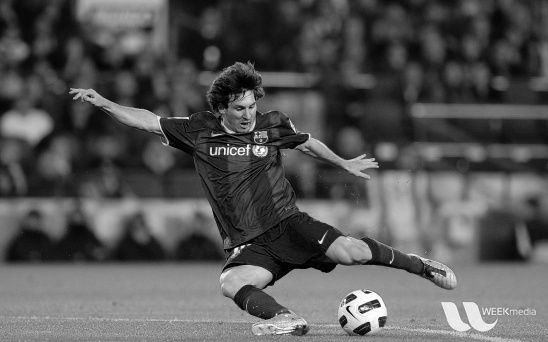
\includegraphics[height=40mm]{green}}
\fbox{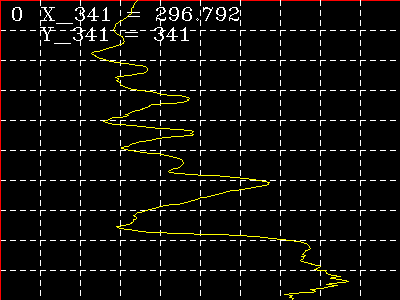
\includegraphics[height=40mm]{projection}}

\bigskip
\noindent%
\fbox{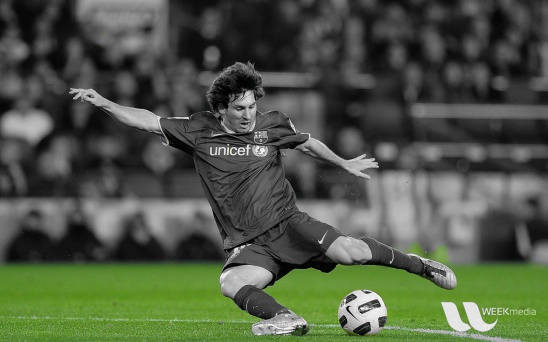
\includegraphics[height=40mm]{grass}}
\fbox{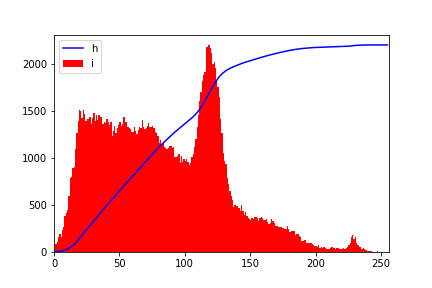
\includegraphics[height=40mm]{histogram}}


\section{Submitting the report}

When you have answered to the questions in Section~\ref{sec:running},
inserted the code in Section~\ref{sec:code} and verified that the
four generated images are visible in Section~\ref{sec:images}, send
the PDF by email to \texttt{jorma.laaksonen@aalto.fi}

Welcome to the course starting 14.5.2018 at 9:15 o'clock in lecture
hall Exactum B222!

\end{document}
%  LocalWords:  Jorma Laaksonen pdf py tex OpenCV libopencv dev jpg
%  LocalWords:  highgui imgproc imgcodecs greyscale png opencv ing
%  LocalWords:  texlive includegraphics Exactum Gür Ersalan
